% Prezentacja - etap 3 (28.X): projekt wstępny systemu.
% Kompilacja (XeLaTeX):  tectonic prezentacja.tex   (albo ../../prezentacja/build.sh nie dotyczy etapu 3)
\documentclass[aspectratio=169,11pt]{beamer}

\usetheme[progressbar=frametitle,numbering=fraction]{metropolis}
\usepackage[polish]{babel}
\usepackage{booktabs}
\usepackage{tabularx}
\usepackage{listings}
\usepackage{xcolor}
\usepackage{amssymb}
\usepackage{tikz}
\usetikzlibrary{arrows.meta,positioning}

\graphicspath{{../diagramy/}{img/}}
\newcolumntype{L}{>{\raggedright\arraybackslash}X}

\definecolor{ok}{HTML}{11804B}
\definecolor{bad}{HTML}{C0392B}
\definecolor{warn}{HTML}{A15C00}
\definecolor{acc}{HTML}{1F5EFF}
\newcommand{\good}[1]{\textcolor{ok}{#1}}
\newcommand{\bad}[1]{\textcolor{bad}{#1}}

\lstset{
  basicstyle=\ttfamily\footnotesize,
  keywordstyle=\color{acc}\bfseries,
  commentstyle=\color{gray},
  language=Python,
  columns=fullflexible,
  keepspaces=true,
  frame=none,
  backgroundcolor=\color{black!4},
  xleftmargin=4pt, framexleftmargin=4pt,
  extendedchars=true,
  literate={ą}{{\k{a}}}1 {ę}{{\k{e}}}1 {ó}{{\'o}}1 {ś}{{\'s}}1 {ł}{{\l}}1 {ż}{{\.z}}1 {ź}{{\'z}}1 {ć}{{\'c}}1 {ń}{{\'n}}1,
}

% pełnoekranowy diagram
\newcommand{\fullimage}[2][0.98]{%
  \begin{frame}[plain]
    \begin{tikzpicture}[remember picture, overlay]
      \node at (current page.center) {\includegraphics[width=0.99\paperwidth,height=#1\paperheight,keepaspectratio]{#2}};
    \end{tikzpicture}
  \end{frame}}

\title{System zapisów na zajęcia -- USOSv2}
\subtitle{Etap 3: projekt wstępny systemu}
\author{Kamil Kręcigłowa \and Bartosz Królik \and Krzysztof Krówka}
\institute{Inżynieria Oprogramowania, zima 2026/2027}
\date{28 października 2026}

\begin{document}

\maketitle

% ---------------------------------------------------------------------------
\begin{frame}{Co jest w etapie 3}
  \begin{columns}[T]
    \begin{column}{0.48\textwidth}
      \textbf{Zakres (z opisu zadania)}
      \begin{itemize}\small
        \item architektura i stos technologiczny
        \item przypadki użycia UC0--UC27
        \item diagramy sekwencji -- 7
        \item diagram ER
        \item diagramy klas: metody, parametry, wyniki, opis
      \end{itemize}
      \textbf{Projekt sprawdzony kodem}
      \begin{itemize}\small
        \item diagramy = działająca implementacja
        \item 35 testów, test obciążeniowy 20\,000 kont
      \end{itemize}
    \end{column}
    \begin{column}{0.48\textwidth}
      \textbf{Zmiany względem etapu 2}
      \begin{itemize}\small
        \item \textbf{tury per kierunek} -- ograniczenie ruchu
        \item jedna tabela \texttt{app\_user} z rolą
        \item \textbf{reguły biznesowe w kodzie}, nie w SQL
        \item kontrola ruchu: cache, limity, 503 + Retry-After
        \item ślad decyzji dziekanatu (\texttt{created\_by})
      \end{itemize}
    \end{column}
  \end{columns}
\end{frame}

% ---------------------------------------------------------------------------
\section{Architektura}

\fullimage{architektura.png}

\begin{frame}{Architektura: zasady}
  \begin{columns}[T]
    \begin{column}{0.5\textwidth}
      \small
      \begin{enumerate}
        \item \textbf{Domena bez bazy.} Reguły (kolizje, wymagania, tury, „jedna grupa typu'') to czyste funkcje: dostają dane, zwracają decyzję.
        \item \textbf{Serwis = transakcja.} Blokady $\rightarrow$ dane $\rightarrow$ reguły $\rightarrow$ zapis $\rightarrow$ outbox.
        \item \textbf{Baza = siatka bezpieczeństwa.} \texttt{CHECK}, \texttt{UNIQUE}, FK odrzucą wynik błędu w kodzie.
      \end{enumerate}
    \end{column}
    \begin{column}{0.46\textwidth}
      \small
      \begin{enumerate}\setcounter{enumi}{3}
        \item \textbf{Kolejność blokad} student $\rightarrow$ grupa; awans z listy odwraca ją, więc \texttt{NOWAIT} + ponowienie.
        \item \textbf{Outbox} -- powiadomienie w tej samej transakcji, e-mail wysyła worker.
        \item \textbf{Bezstanowe API} -- skaluje się kolejnymi instancjami.
      \end{enumerate}
      \begin{alertblock}{Dlaczego to ważne}
        Przy refaktoryzacji błąd zdjął blokadę grupy -- \texttt{CHECK} odrzucił 11.\ zapis na 10 miejsc, test go wychwycił.
      \end{alertblock}
    \end{column}
  \end{columns}
\end{frame}

\begin{frame}{Stos technologiczny}
  \scriptsize
  \begin{tabularx}{\textwidth}{@{}l>{\raggedright}p{4.2cm}L@{}}
    \toprule
    \textbf{Element} & \textbf{Technologia} & \textbf{Uzasadnienie} \\
    \midrule
    Frontend & React 19 + TypeScript, Vite & typowanie, katalog, formularze, siatka planu \\
    Serwer WWW & nginx & statyka z cache -- odświeżanie strony nie obciąża API \\
    Backend & Python 3.12, FastAPI, Pydantic & async, walidacja, OpenAPI z kodu \\
    Dostęp do bazy & SQLAlchemy 2 + asyncpg & ORM w panelu; gorąca ścieżka bez ORM (pomiar: ORM = główny koszt CPU) \\
    Baza & PostgreSQL 16 & ACID, \texttt{FOR UPDATE NOWAIT / SKIP LOCKED}, blokady doradcze, indeksy częściowe \\
    Migracje & Alembic & wersjonowany schemat dla grupy przejmującej \\
    W tle & własny worker (asyncio) & tury i outbox w bazie -- broker zbędny \\
    Auth & JWT (12 h), bcrypt & logowanie przed turą, bezstanowe API; docelowo SSO \\
    Testy & pytest na PostgreSQL, k6 & blokady i wyścigi tylko na prawdziwej bazie \\
    Wdrożenie & Docker Compose & to samo środowisko dla obu grup \\
    \bottomrule
  \end{tabularx}
\end{frame}

% ---------------------------------------------------------------------------
\section{Przypadki użycia}

\fullimage{przypadki_uzycia_student.png}
\fullimage{przypadki_uzycia_administracja.png}

\begin{frame}{Przypadki użycia: endpointy i błędy (wybór)}
  \scriptsize
  \begin{tabularx}{\textwidth}{@{}>{\raggedright}p{1.9cm}>{\raggedright}p{5.3cm}L@{}}
    \toprule
    \textbf{UC} & \textbf{Endpoint} & \textbf{Błędy (409 / 429 / 503)} \\
    \midrule
    UC2, 5 {\tiny(student)} & \texttt{POST /api/me/enrollments} & ROUND\_CLOSED, SAME\_KIND, PREREQUISITES, CONFLICT, WAITLIST\_FULL, RATE\_LIMITED, OVERLOADED \\
    UC6, 9 {\tiny(student)} & \texttt{DELETE /api/me/enrollments/\{s\}} & ROUND\_CLOSED, NOT\_ENROLLED \\
    UC10 {\tiny(prowadzący)} & \texttt{GET /api/sections/\{s\}/roster} & FORBIDDEN (cudza grupa) \\
    UC11 {\tiny(dziekanat)} & \texttt{POST /api/admin/courses/\{c\}/prerequisites} & PREREQUISITE\_CYCLE \\
    UC12 {\tiny(dziekanat)} & \texttt{POST /api/admin/sections/\{s\}/meetings} & ROOM\_TOO\_SMALL, ROOM\_BUSY, LECTURER\_BUSY \\
    UC13 {\tiny(dziekanat)} & \texttt{PATCH /api/admin/sections/\{s\}} & BELOW\_ENROLLED, ROOM\_FULL \\
    UC14 {\tiny(dziekanat)} & \texttt{POST /api/admin/enrollments} & ALREADY\_ENROLLED, CONFLICT, SAME\_KIND, ROOM\_FULL \\
    UC16, 23 {\tiny(dziekanat)} & \texttt{POST /api/admin/rounds}, \texttt{…/\{r\}/open|close} & BAD\_DATES \\
    \bottomrule
  \end{tabularx}

  \footnotesize Pełna tabela UC0--UC27: \texttt{etap3/README.md}, sekcja 4.
\end{frame}

\begin{frame}{Uprawnienia ról i obsługa błędów}
  \begin{columns}[T]
    \begin{column}{0.5\textwidth}
      \footnotesize
      \begin{tabular}{@{}lccc@{}}
        \toprule
        & \textbf{Stud.} & \textbf{Prow.} & \textbf{Dziek.} \\
        \midrule
        katalog & \good{$\checkmark$} & \good{$\checkmark$} & \good{$\checkmark$} \\
        własne zapisy, plan, listy & \good{$\checkmark$} & -- & -- \\
        listy studentów grupy & -- & swoje & \good{$\checkmark$} \\
        katalog, harmonogram, limity & -- & -- & \good{$\checkmark$} \\
        decyzje o zapisach & -- & -- & \good{$\checkmark$} \\
        tury, konta, oceny, audyt & -- & -- & \good{$\checkmark$} \\
        \bottomrule
      \end{tabular}\\[6pt]
      Student nie podaje \texttt{student\_id} -- id pochodzi z tokenu.
    \end{column}
    \begin{column}{0.46\textwidth}
      \footnotesize
      Każdy błąd: \texttt{\{code, message, details\}}
      \begin{itemize}
        \item \textbf{409} -- odmowa z powodem (\emph{„Kolizja w planie z: BD L05''})
        \item \textbf{429 / 503} + \texttt{Retry-After} -- SPA ponawia sama, z rozrzutem
        \item \textbf{401 / 403 / 404 / 422}
        \item deadlock, \texttt{NOWAIT} -- ponawiane w transakcji, użytkownik ich nie widzi
      \end{itemize}
    \end{column}
  \end{columns}
\end{frame}

% ---------------------------------------------------------------------------
\section{Diagramy sekwencji}

\fullimage{sekwencja_zapis.png}
\fullimage{sekwencja_wypis_awans.png}
\fullimage{sekwencja_tura.png}
\fullimage{sekwencja_dziekanat.png}
\fullimage{sekwencja_harmonogram.png}
\fullimage{sekwencja_wymagania_import.png}
\fullimage{sekwencja_logowanie.png}

% ---------------------------------------------------------------------------
\section{Model danych}

\fullimage{er.pdf}

\begin{frame}{Model danych: co nowe}
  \begin{columns}[T]
    \begin{column}{0.52\textwidth}
      \small
      \begin{itemize}
        \item \texttt{program} -- kierunek studenta i tur
        \item \texttt{round\_program} -- tura obejmuje wybrane kierunki; bez wierszy = wszyscy; tury mogą się nakładać
        \item \texttt{app\_user} -- jedna tabela, dane roli z \texttt{CHECK}
        \item \texttt{enrollment.created\_by / dropped\_by} -- kto z dziekanatu
        \item \texttt{notification.read\_at, attempts}
      \end{itemize}
    \end{column}
    \begin{column}{0.44\textwidth}
      \small
      \textbf{Bez zmian z etapu 2:} kurs $\neq$ grupa, terminy w \texttt{meeting}, licznik \texttt{enrolled\_count} + \texttt{CHECK}, historia zamiast kasowania, kolejność listy = \texttt{id}, outbox.\\[6pt]
      \textbf{Usunięte z bazy:} funkcje kolizji, trigger cykli, widok audytu -- przeniesione do kodu.
    \end{column}
  \end{columns}
\end{frame}

% ---------------------------------------------------------------------------
\section{Projekt klas}

\fullimage{klasy_domena.png}

\begin{frame}{Domena: kluczowe operacje}
  \scriptsize
  \begin{tabularx}{\textwidth}{@{}>{\raggedright}p{5.4cm}>{\raggedright}p{3.0cm}L@{}}
    \toprule
    \textbf{Operacja} & \textbf{Zwraca} & \textbf{Funkcjonalność} \\
    \midrule
    \texttt{check\_student(student: StudentState, target: TargetSection, mode: Mode)} & \texttt{list[Refusal]} & powody odmowy: tura, już zapisany/czeka, typ grupy, wymagania, kolizje \\
    \texttt{decide\_seat(seat: SeatState, mode: Mode)} & \texttt{Outcome | Refusal} & ENROLL / WAITLIST / ENROLL\_OVER\_CAPACITY (dziekanat, $\le$ sala) / odmowa \\
    \texttt{conflicting\_sections(plan, new: Iterable[Slot])} & \texttt{list[Scheduled\-Section]} & dzień, godziny (styk to nie kolizja), parzystość tygodni \\
    \texttt{creates\_cycle(graph, course\_id, required\_id)} & \texttt{bool} & czy nowe wymaganie zamknie cykl \\
    \texttt{student\_can\_enroll(rounds, program\_id)} & \texttt{bool} & otwarta tura obejmuje kierunek \\
    \texttt{scheduled\_transition(round, now)} & \texttt{"OPEN" | "CLOSED" | None} & harmonogram tur dla workera \\
    \bottomrule
  \end{tabularx}
  \vspace{2pt}

  \footnotesize W serwisie: \texttt{check\_student} (blokada studenta) $\rightarrow$ 409 albo blokada grupy $\rightarrow$ \texttt{decide\_seat} $\rightarrow$ zapis.
\end{frame}

\fullimage{klasy_serwisy.png}

\begin{frame}{EnrollmentService: operacje}
  \scriptsize
  \begin{tabularx}{\textwidth}{@{}>{\raggedright}p{6.2cm}>{\raggedright}p{2.6cm}L@{}}
    \toprule
    \textbf{Operacja} (\texttt{s: AsyncSession} pominięte) & \textbf{Zwraca} & \textbf{Funkcjonalność} \\
    \midrule
    \texttt{enroll(student\_id, section\_id, mode=DIRECT, actor\_id=None)} & \texttt{EnrollResult} & UC2/5/14: blokady, reguły, zapis albo lista, anulowanie list tego typu \\
    \texttt{drop(student\_id, section\_id, mode=DIRECT, actor\_id=None)} & \texttt{list[PromotionEvent]} & UC6/14: wypis (student tylko w turze), potem awans \\
    \texttt{leave\_waitlist(student\_id, section\_id)} & \texttt{None} & UC7 \\
    \texttt{change\_limits(section\_id, capacity=None, waitlist\_limit=None)} & \texttt{list[PromotionEvent]} & UC13: zapisani $\le$ limit $\le$ sala, potem awans \\
    \texttt{promote(section, target, term\_id)} & \texttt{list[PromotionEvent]} & UC9: dopóki są miejsca -- \texttt{NOWAIT}, ponowne reguły, PROMOTED / SKIPPED \\
    \texttt{waitlist\_position(student\_id, section\_id)} & \texttt{int | None} & pozycja na liście \\
    \bottomrule
  \end{tabularx}
  \vspace{6pt}

  \footnotesize Pozostałe serwisy (Catalog, Rounds, Users, Records, Notification, Audit, Query) i \texttt{Loaders} -- tabele z opisem każdej metody w \texttt{etap3/README.md}, sekcja 7.
\end{frame}

\fullimage{klasy_infrastruktura.png}

% ---------------------------------------------------------------------------
\section{Duży ruch}

\begin{frame}{20\,000 studentów: ograniczyć ruch, potem go obsłużyć}
  \begin{columns}[T]
    \begin{column}{0.5\textwidth}
      \small
      \textbf{1. Tury per kierunek (UC23)}\\
      kolejny kierunek co 30 min $\Rightarrow$ w szczycie ok.\ 1000 osób zamiast 20\,000.\\[6pt]
      \textbf{2. Krótkie blokady}\\
      reguły planu studenta przed blokadą grupy; pod blokadą grupy tylko kilka zapytań.\\[6pt]
      \textbf{3. Kontrola wejścia}\\
      limit operacji na studenta (429), bramka równoczesnych transakcji (503 + \texttt{Retry-After}), SPA ponawia z rozrzutem.
    \end{column}
    \begin{column}{0.46\textwidth}
      \small
      \textbf{4. Cache odczytów}\\
      katalog 3\,s (równoczesne chybienia = jedno zapytanie), dane grupy przy zapisie 10\,s.\\[6pt]
      \textbf{5. Gorąca ścieżka bez ORM}\\
      profilowanie: budowanie zapytań w SQLAlchemy zjadało CPU $\Rightarrow$ asyncpg.\\[6pt]
      \textbf{6. Skalowanie}\\
      API bezstanowe, statyka z nginx, logowanie przed turą (JWT 12\,h).
    \end{column}
  \end{columns}
\end{frame}

\begin{frame}{Test obciążeniowy: otwarcie tury (k6)}
  \small
  Każdy student: katalog, status grup, zapis na 6 przedmiotów (wykład + laboratorium), plan.
  Seed: 20 kierunków, 20\,000 kont, 9000 grup. Jedna maszyna (16 rdzeni) razem z k6.\\[2pt]
  \footnotesize
  \begin{tabularx}{\textwidth}{@{}L>{\raggedleft}p{1.7cm}>{\raggedleft}p{1.9cm}>{\raggedleft}p{2.8cm}>{\raggedleft\arraybackslash}p{2.4cm}@{}}
    \toprule
    \textbf{Scenariusz} & \textbf{p95 zapisu} & \textbf{sesja studenta} & \textbf{ponowienia 429/503} & \textbf{niezmienniki} \\
    \midrule
    1 kierunek, 1000 osób -- pierwsza wersja & 2,5\,s & 2\,min & \bad{22\,873 (1576 nieudanych)} & \good{OK} \\
    1 kierunek, 1000 osób -- po poprawkach & \good{1,9\,s} & \good{17\,s} & \good{0} & \good{OK} \\
    3 kierunki, 3000 osób (przeciążenie) & 2,1\,s & 49\,s & 18\,034 (0,5\,\% nieudanych) & \good{OK, 0 przepełnień} \\
    \bottomrule
  \end{tabularx}\\[4pt]
  \footnotesize
  \begin{itemize}
    \item wąskie gardło: CPU procesów API (baza ok.\ 1/4 mocy) $\Rightarrow$ kolejne instancje API
    \item pierwsza wersja: limit liczył też ponowienia $\Rightarrow$ kaskada 429 -- znalezione dopiero pomiarem
    \item przeciążenie: system zwalnia, ale \textbf{nie traci spójności} $\Rightarrow$ tury per kierunek są konieczne
  \end{itemize}
\end{frame}

\begin{frame}{Implementacja: ekrany}
  \begin{columns}[T]
    \begin{column}{0.5\textwidth}
      \centering
      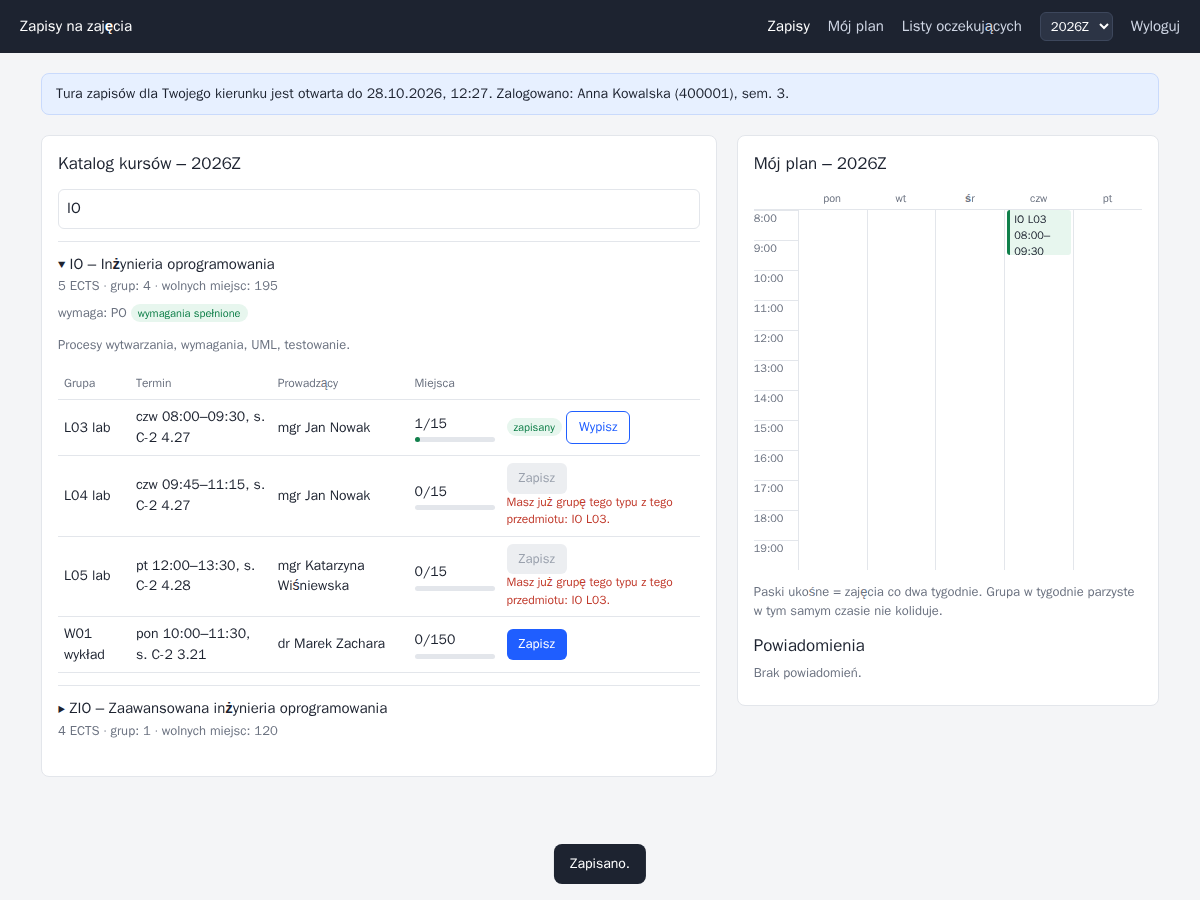
\includegraphics[width=\textwidth]{student_zapisy.png}\\
      \footnotesize student: status grup z powodem odmowy, plan, tura kierunku
    \end{column}
    \begin{column}{0.5\textwidth}
      \centering
      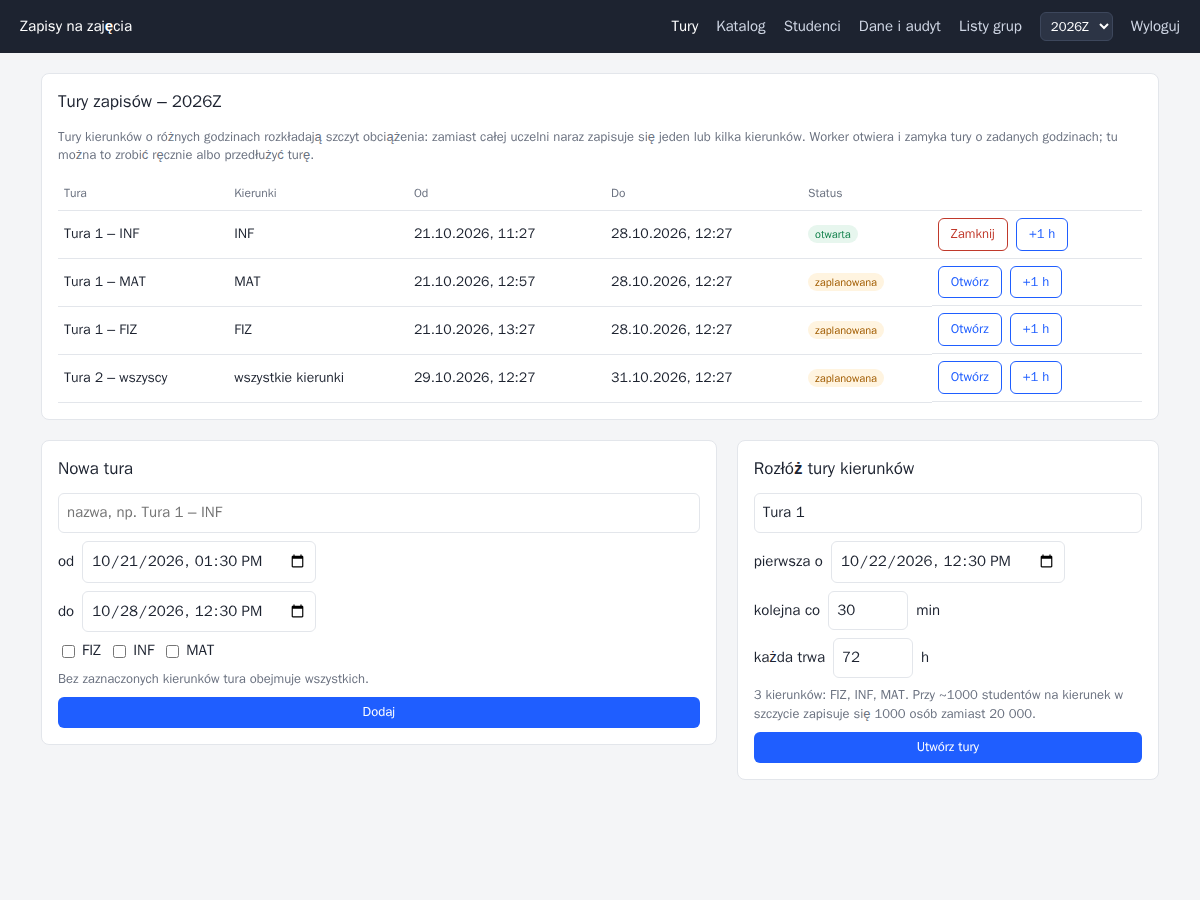
\includegraphics[width=\textwidth]{dziekanat_tury.png}\\
      \footnotesize dziekanat: tury kierunków, „Rozłóż tury kierunków''
    \end{column}
  \end{columns}
\end{frame}

% ---------------------------------------------------------------------------
\section{Podsumowanie}

\begin{frame}{Weryfikacja i przekazanie projektu}
  \begin{columns}[T]
    \begin{column}{0.5\textwidth}
      \small
      \textbf{Weryfikacja}
      \begin{itemize}
        \item 35 testów na PostgreSQL: reguły, wyścigi (30 osób / 10 miejsc, dwie karty, awans vs zapis -- ścieżka \texttt{NOWAIT} faktycznie wykonywana), API, worker
        \item test obciążeniowy + audyt niezmienników po teście
      \end{itemize}
    \end{column}
    \begin{column}{0.46\textwidth}
      \small
      \textbf{Dla grupy przejmującej}
      \begin{itemize}
        \item \texttt{docker compose up} + seed demo/uczelnia
        \item nowa reguła $\rightarrow$ \texttt{app/domain} + test
        \item zmiana schematu $\rightarrow$ migracja Alembic
        \item znane ograniczenia: kursy nieprzypisane do kierunków, brak zamiany grupy, limit per proces, jedna rola na konto
      \end{itemize}
    \end{column}
  \end{columns}
\end{frame}

\begin{frame}[standout]
  Dziękujemy\\[6pt]
  \normalsize Pytania?
\end{frame}

\end{document}
